\documentclass[10pt,a4paper,twocolumn]{article}
\usepackage[T1]{fontenc}
\usepackage[utf8]{inputenc}
\usepackage{times}
\usepackage[a4paper,top=2.2cm,bottom=2.4cm,left=2cm,right=2cm,columnsep=0.8cm]{geometry}
\usepackage{booktabs}
\usepackage{graphicx}
\usepackage{stfloats}
\usepackage{balance}
\usepackage{microtype}
\usepackage[hidelinks]{hyperref}
\usepackage{enumitem}
\setlist{nosep,leftmargin=*}
\setlength{\parskip}{0pt}
\usepackage{titlesec}
\titlespacing*{\section}{0pt}{10pt plus 2pt}{4pt}
\titleformat{\section}{\normalfont\large\bfseries}{\thesection}{0.6em}{}
\renewcommand{\paragraph}[1]{\par\textbf{#1}\ }
\usepackage{caption}
\captionsetup{font=small,labelfont=bf,skip=4pt}
\setlength{\textfloatsep}{10pt plus 2pt}
\setlength{\dbltextfloatsep}{10pt plus 2pt}

\title{\vspace{-1.0cm}\Large\textbf{Compress the Prose, Not the Language: Linguistic Redundancy}\\[2pt]
\Large\textbf{in Memorization and Reasoning of Small Transformers}}
\author{Marco COGNOME\\ \small Independent researcher\\ \small ORCID: 0009-0004-2917-4466}
\date{\small November 2026}

\begin{document}
\twocolumn[
\maketitle
\vspace{-0.6cm}
\begin{center}
\begin{minipage}{0.88\textwidth}
\small
\textbf{Abstract.} Natural language carries redundancy (function words, agreement, restatement) that looks superfluous to a model. We ask whether removing it lets transformers store the same facts with fewer parameters, train faster, or reason with fewer tokens. In a controlled memorization setting (20,000 synthetic biographies, models trained from scratch at 0.15--8M parameters), compression does not change the capacity needed at saturation, which is set by the facts (about 1--2 bits per parameter). It shortens training to 0.55--0.86$\times$ the time, and lowers parameters mid-curve only when the compressed form is regular and keeps the words that distinguish relations. In reasoning (GSM8K, Qwen3 0.6B/1.7B/4B with LoRA), designed formats (telegraphic stripping, a canonical equation language) lose 2--4 accuracy points at every scale. Concise natural prose instead matches full chain-of-thought accuracy with 25--26\% fewer tokens and up to 27\% lower latency. Filler can be removed; numbers and relational words carry the information.
\end{minipage}
\end{center}
\vspace{0.4cm}
]

\section{Introduction}
A reader recovers ``I am going to do the shopping'' from ``go shopping''. Printed language is highly redundant~[1], and speakers drop predictable material when information density allows~[2]. For a language model every token costs compute, so two ideas are tempting: strip predictable words before training, or translate text into a compact, language-free interlingua. We test both empirically and ask:
\begin{itemize}
\item \textbf{RQ1 Capacity.} Does compressed text need fewer parameters to store the same facts?
\item \textbf{RQ2 Compute.} Does it reduce training and inference cost?
\item \textbf{RQ3 Reasoning.} Can a pretrained model reason in a compressed form without losing accuracy?
\end{itemize}
Our contributions are a controlled 2$\times$2 design that separates regularity of form from word removal, a seven-iteration study with paired tests across three model scales, and a practical finding: concise natural prose is the best compression we found.

\section{Related work}
Information-theoretic accounts treat redundancy as predictability in context~[1,2]. Allen-Zhu and Li show that transformers store about 2 bits of factual knowledge per parameter after sufficient exposure, on synthetic biographies similar to ours~[3]. LLMLingua compresses prompts by dropping low-surprisal tokens with a small model~[4]; Chain of Draft prompts models to write minimal reasoning steps~[5] in place of verbose chain-of-thought~[6]. These works compress at inference time; we instead train on compressed formats and isolate why compression helps or hurts.

\section{Experimental setup}
\paragraph{Part I: memorization from scratch.} We generate 20,000 unique fictional persons with six attributes (birth date, birth city, university, field, profession, employer), about 49 bits per person and 1\,Mbit in total. Each biography is written in Italian in several formats: full prose with 4 templates per attribute and pronouns; telegraphic, with function words removed; an interlingua with fixed attribute markers; a rich variant with 10+ templates and filler; and a canonical variant with one template per attribute. Decoder-only transformers (0.15--8M non-embedding parameters) are trained from scratch with a per-format BPE tokenizer and 200 exposures per biography. All formats receive the same number of optimizer steps: at equal exposures shorter text gets fewer updates, which in our first run inflated the parameters needed by compressed formats 1.45--2.0$\times$. We measure exact-match recall of each attribute from a native prompt and interpolate the parameters needed for 50\% and 90\% recall (2--3 seeds).

\paragraph{Part II: reasoning in pretrained models.} On GSM8K~[7] (6,381 training and 1,319 test problems), a local Qwen3-4B-Instruct rewrites each official solution into several formats. A rewrite is kept only if its final answer and all official intermediate results are preserved. The formats are full prose (A); telegraphic (B, list-based stripping); a canonical line language \texttt{name = expr = value} (C); concise prose with one short sentence per step and relational words kept (A1); very concise prose of at most 8 words per step (A2); and answer only (D). We fine-tune Qwen3-0.6B/1.7B-Base~[9] with LoRA~[8] ($r{=}16$, 2 epochs, identical steps; 3 and 2 seeds) and Qwen3-4B-Base with QLoRA~[10] (1 seed). Decoding is greedy, optionally with a calculator that forces arithmetic results and, for C, grammar-constrained decoding. Formats are compared with paired McNemar tests.


\section{Results I: memorization}
Compression changes how fast facts are learned, not how many parameters they need. Peak storage is 1.6--2.2 bits per parameter at 200 exposures and about 3 at 500, close to~[3]. At 90\% recall every format needs 0.95--1.01$\times$ the parameters of full prose (Table~\ref{tab:2x2}).

\begin{table}[!htb]
\centering\small
\caption{Total parameters needed, relative to full varied prose (BPE 2048, 3 seeds; 95\% bootstrap CI).}
\label{tab:2x2}
\begin{tabular}{@{}lccc@{}}
\toprule
Format & Tok/bio & @50\% & @90\% \\
\midrule
Full, varied (4 templ.) & 57.6 & 1.00 & 1.00 \\
Full, canonical (1 templ.) & 55.8 & 0.91 & 1.01 \\
Stripped, varied & 40.5 & 1.05 & 0.98 \\
Stripped, canonical & 41.5 & \textbf{0.85} & 0.95 \\
 & & {\scriptsize [0.83--0.87]} & {\scriptsize [0.92--1.01]} \\
\bottomrule
\end{tabular}
\end{table}


At 50\% recall, regularity explains about 97\% of the gain (Shapley decomposition in log space). Stripping helps only once forms are canonical (interaction 0.89 [0.85--0.94]). Stripping varied text makes 75\% of birth-date and birth-place sentences share a prefix (\emph{``è nato il / a''} $\rightarrow$ \emph{``nato''}): removing one preposition merged two relations. The last fact learned, the 14-bit birth date, sets the 90\% threshold and benefits from neither factor.

The robust gain is compute. Time to 90\% recall falls to 0.55$\times$ (stripped canonical), 0.66$\times$ (stripped varied) and 0.86$\times$ (canonical). With fewer exposures (100 instead of 200) the telegraphic format needs 0.69$\times$ the parameters for 50\% recall, a learning-speed effect that vanishes with longer training. Two further checks: shrinking the vocabulary from 4,096 to 1,024--2,048 cuts total parameters by 18--21\% for every format, leaving the compressed/full ratio at 0.86--0.93; and a bilingual Italian/English corpus needs no extra parameters (0.94--0.96$\times$) but shows no cross-lingual transfer for translated values (1--3\% recall at 4M), so facts are stored as string associations rather than language-free concepts. For short factual answers, a rule-based strip/realize pipeline runs at 0.96--1.00$\times$ the latency of the full-prose model: there is nothing to save, since the answer is the same value in every format.

\section{Results II: reasoning}
Concise prose (A1) keeps full-prose accuracy at three quarters of the tokens; the canonical language (C) pays 3.4--4.0 points at the same length, at every scale (Table~\ref{tab:gsm}, Figure~\ref{fig:frontier}).

\begin{figure*}[!b]
\centering
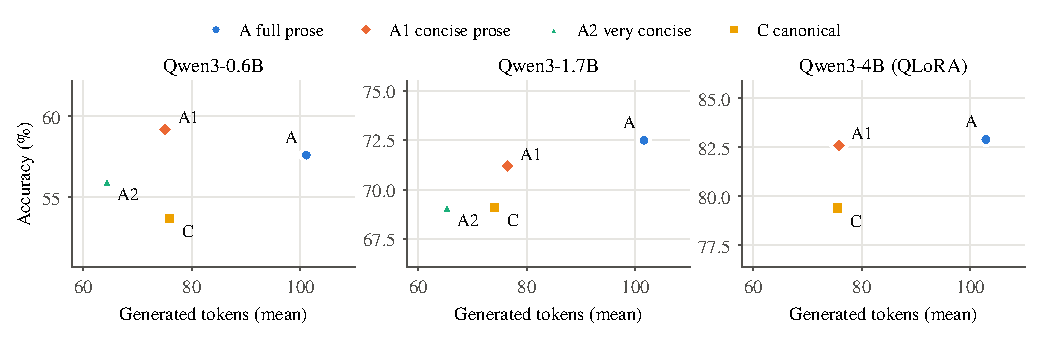
\includegraphics[width=0.92\textwidth]{fig_frontier.pdf}
\caption{GSM8K accuracy versus mean generated tokens, one panel per model (all formats with calculator; C also grammar-constrained). A1 sits at A's accuracy with C's length; C and A2 lose accuracy at similar or shorter lengths.}
\label{fig:frontier}
\end{figure*}

\begin{table}[!htb]
\centering\small
\setlength{\tabcolsep}{4pt}
\caption{GSM8K test accuracy (\%) / mean generated tokens, with calculator (C also grammar-constrained). Seeds: 3 (0.6B), 2 (1.7B), 1 (4B, QLoRA).}
\label{tab:gsm}
\begin{tabular}{@{}lccc@{}}
\toprule
Format & 0.6B & 1.7B & 4B \\
\midrule
A full prose & 57.6/101 & 72.5/102 & 82.9/103 \\
A1 concise prose & \textbf{59.2}/75 & 71.2/76 & 82.6/76 \\
A2 very concise & 56.0/64 & 69.1/65 & -- \\
C canonical lang. & 53.7/76 & 69.1/74 & 79.4/76 \\
D answer only$^\dagger$ & 16.4/3 & 23.5/3 & -- \\
\bottomrule
\end{tabular}\\[1pt]
{\scriptsize $^\dagger$without calculator.}
\end{table}


At equal length, A1 beats C by 5.5 ($p<10^{-11}$), 2.1 ($p=0.03$) and 3.3 points ($p=0.006$). Against A, A1 differs by +1.5 ($p=0.04$, unstable across seeds), $-1.3$ ($p=0.12$) and $-0.2$ points ($p=0.88$). Telegraphic stripping (B, without calculator) saves only 12--13\% of tokens and loses 1.4--2.6 points. The floor is the digits: Qwen3 tokenizes each digit separately, so equations and the answer line make up about 49\% of A's tokens.

Why designed formats lose:
\begin{itemize}
\item \textbf{No recovery.} Without a calculator, when at least one equation is wrong the final answer is still correct in 24\%/43\% of A outputs (0.6B/1.7B), 17\%/30\% for A1 and only 7\%/9\% for C.
\item \textbf{Fixes do not close the gap.} Grammar-constrained decoding costs 0.9--1.1 points: every problem it lost had been solved by an output that broke the grammar. The calculator adds 1.0--2.2 points to C but also helps A. Unit-suffixed variable names and an equation-solving line cost a further 1.5--2.4 points.
\item \textbf{Ambiguity moves, it does not disappear.} In 20 sampled errors per condition, format-induced errors number 0/20 for A1, 12/20 for A2 and 13/40 for C: unlabeled numbers, names that misstate their quantity, percentages read as dollars.
\end{itemize}
Latency follows token count (about 15--17\,ms per token): A1 answers 23\% faster than A at 0.6B and 27\% faster at 4B (batch 1).

\section{Discussion and limitations}
The two settings agree on what carries information: entities and numbers, which set an incompressible floor, and the small words that state how quantities relate (\emph{of, each, per, from}; \emph{il} versus \emph{a}). These words look like function words, yet removing them merged relations in every experiment, from birth dates to discounts. Filler, restatement and transition sentences can be deleted at no measurable cost. For a pretrained model, grammar is not filler either: it is the model's native code and acts as error-correcting redundancy. Every designed format failed the same way, with each fix opening a new channel of ambiguity (prefix collisions, then variable names, then units).

\paragraph{Limitations.} Models are small (at most 4B parameters) and trained on a consumer GPU (RTX 4070 SUPER); seeds are few (one at 4B, run with 4-bit QLoRA). Part I uses synthetic Italian biographies with independent attributes, so it measures storage, not comprehension. Part II covers one English task; its rewrites come from a 4B model of the same family, and A1/A2 were kept by a soft length criterion. GSM8K may appear in pretraining data, equally for all formats. Error categories were assigned by an LLM on 20 samples per condition. Latencies are dominated by per-step overhead, so token counts are the more reliable cost measure.

\section{Conclusion}
Removing words does not shrink what a model must store; it only makes text cheaper to process. The safe compression deletes filler and keeps relational words: concise prose matched full chain-of-thought at 75\% of the tokens across three scales, while every designed format lost 2--4 points. In practice, asking a model to reason in short sentences, one step per line, without restating the question and keeping connectives, saves about a quarter of the reasoning tokens.

\paragraph{AI use.} Experiments were implemented and run with an AI coding agent (Claude Code), and the manuscript was drafted with AI assistance. The author designed the study, reviewed all results and takes full responsibility for the content.
\paragraph{Reproducibility.} Code, generated data and per-problem outputs are available at \url{https://github.com/adapt-to-it/lingcompress} (DOI: 10.5281/zenodo.XXXXXXX).

\balance
{\small
\section*{References}
\begin{enumerate}[label={[\arabic*]},leftmargin=1.6em]
\item C.~E. Shannon. Prediction and entropy of printed English. \emph{Bell System Technical Journal}, 30(1):50--64, 1951.
\item T.~F. Jaeger. Redundancy and reduction: Speakers manage syntactic information density. \emph{Cognitive Psychology}, 61(1):23--62, 2010.
\item Z.~Allen-Zhu and Y.~Li. Physics of language models: Part 3.3, knowledge capacity scaling laws. In \emph{ICLR}, 2025. arXiv:2404.05405.
\item H.~Jiang, Q.~Wu, C.-Y. Lin, Y.~Yang and L.~Qiu. LLMLingua: Compressing prompts for accelerated inference of large language models. In \emph{EMNLP}, pp.~13358--13376, 2023.
\item S.~Xu, W.~Xie, L.~Zhao and P.~He. Chain of Draft: Thinking faster by writing less. arXiv:2502.18600, 2025.
\item J.~Wei et al. Chain-of-thought prompting elicits reasoning in large language models. In \emph{NeurIPS}, 2022.
\item K.~Cobbe et al. Training verifiers to solve math word problems. arXiv:2110.14168, 2021.
\item E.~J. Hu et al. LoRA: Low-rank adaptation of large language models. In \emph{ICLR}, 2022.
\item Qwen Team (A.~Yang et al.). Qwen3 technical report. arXiv:2505.09388, 2025.
\item T.~Dettmers, A.~Pagnoni, A.~Holtzman and L.~Zettlemoyer. QLoRA: Efficient finetuning of quantized LLMs. In \emph{NeurIPS}, 2023.
\end{enumerate}
}
\end{document}
